%
% brechungsgesetz.tex
%
% (c) 2019 Prof Dr Andreas Müller, Hochschule Rapperswil
%
\subsection{Das Brechungsgesetz\label{mo:subsection:brechungsgesetz}}
\begin{figure}
\centering
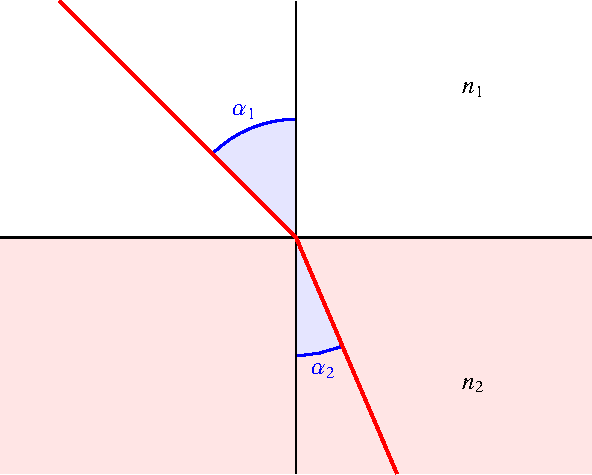
\includegraphics{applications/matrixoptik/snellius.pdf}
\caption{Brechungsgesetz von Snellius
\label{mo:snellius}}
\end{figure}
Das Brechungsgesetz von Snellius beschreibt, wie ein Lichtstrahl beim
\index{Snellius, Brechungsgesetz}
\index{Brechungsgesetz von Snellius}
Eintritt in ein Medium mit einer höheren optischen Dichte gebrochen
wird.
Die {\em optische Dichte} oder {\em Brechungsindex} eines Mediums gibt an,
wie viel langsamer 
\index{optische Dichte}
\index{Brechungszahl}
sich Licht darin bewegt im Vergleich zur Lichtgeschwindigkeit.
Typische optische Glassorten haben einen Brechungsindex zwischen
1.45 und 1.9.

Misst man den Winkel zwischen einem Lichtstrahl und der Normalen auf
die Grenzfläche der Medien wie in Abbildung~\ref{mo:snellius}
dargestellt, dann verhalten sich die Sinus-Werte dieser Winkel
umgekehrt zu den Brechungsindizes, in Formeln
\begin{equation}
\frac{\sin \alpha_1}{\sin\alpha_2} = \frac{n_2}{n_1}.
\label{mo:eq:snellius}
\end{equation}
Der Brechungsindex in Luft ist mit $1.000292$ sehr nahe bei $1$, so
dass für alle praktischen Zwecke der für Luft der Brechungsindex als
$1$ angenommen werden kann.





